%************************************************
\chapter{Introduction}
\label{ch_intro}
\acresetall
%************************************************

Over the past decade, the comparative analysis of genomic sequences
has immeasurably expanded our understanding of the evoluion, biology
and diversity of mammals, the taxonomic class to which we belong.
%\citep{Lander2001,Mouse2002Initial,Rat2004Genome,LindbladToh2005Genome,
% Sequencing2005a,Margulies2007}.  Although the revolution in genomic
medicine that was optimistically predicted during the unveiling of the
draft human genome sequence is still far from being realized
\citep{Collins2001,Varmus2010}, the impact of comparative genomics on
the study of human evolution, diversity and biology has been more
immediate, far-reaching and deep \citep{OBrien1999,Lander2011}. Many
important questions in evolution have been asked---for example, what
is the rate of mammalian speciation
\citep{BinindaEmonds2007,Venditti2011}, or what is the fraction of the
genome under functional constraint
\citep{Boffelli2003a,Siepel2005,Ponting2011}---and, to some extent,
answered using large amounts of genomic data.

The aim of this thesis is to show how the large-scale comparative
analysis of genes and genomes can be used to identify genomic regions
and biological features which have been subject to exceptional levels
of selective constraint throughout mammalian evolution. When shared
across many species, certain evolutionary patterns can highlight genes
and pathways involved in ongoing, universal mammalian genetic
conflicts---for instance, genes related to host immune defense and
reproduction \citep{CastilloDavis2004}. On the other hand, when strong
selective pressures are observed in just one or a few lineages, they
may indicate more specific adaptations related to those species'
unique evolutionary history
\citep{Messier1997,Sawyer2005a,Nielsen2007}.

Along with the increased use of high-throughput methods and datasets
in biology has come a heightened awareness of the inescapable presence
of noise and error within data. The study of genome sequences is no
exception to this point; indeed, the many potential sources of error
in any comparative genomic analysis may combine to make it difficult
to assess accuracy or to distinguish anomalous results from
interesting biological signals
\citep{Mallick2009,Schneider2009,Fletcher2010,MarkovaRaina2011}. Some
of the difficulty of assessing results stems from a limited
understanding of how various sources of error can impact downstream
evolutionary analyses; thus, a secondary aim of this thesis is to
contribute to our understanding of the impact of some sources of error
on large-scale comparative analyses and to further develop methods for
appropriately predicting and handling such error.

\bresp{Hypothesis}A major hypothesis underlying the work described in
this thesis is the idea that a fine-scale comparison of differences in
the evolutionary rates of genes---both within genomes (i.e.\ between
different genes) and across evolutionary histories (i.e.\ between
different species groups)---can be used to identify distinct
biological features and patterns related to the impact of natural
selection on the molecular evolution of proteins in mammals. Following
from this hypothesis, some major points of consideration include the
question of whether errors in genome-scale analysis methods reduce our
ability to detect such features with reasonable accuracy (as
investigated in Chapters \ref{ch_indels1} and \ref{ch_mammals1}),
whether heterogeneous evolutionary patterns in genes can be suitably
and reliably summarized to identify genes with the strongest evidence
of long-term adaptive evolution (as explored in Chapter
\ref{ch_mammals2}), and whether there is sufficient signal within
fixed protein-coding differences to shed light on unique adaptive
events experienced by different primates and mammals (considered in
Chapters \ref{ch_mammals1} and \ref{ch_gorilla}). Each of these topics
is quite broad, with a relatively distinct sub-field devoted to the
development of better models and an improved understanding, but they
together feed into the overall question of whether data from across
dozens of genomes can be successfully used to gather a global picture
of the impact of long-term adaptive evolution on mammalian
genes. \eresp{Hypothesis}

Although each subsequent chapter contains its own short introduction,
this chapter presents some of the key concepts and methods which are
recurrent throughout the thesis or provide an appropriate historical
background. Section \ref{section_mammal_evolution} first introduces
the biology and evolution of the mammals, highlighting features of
their evolutionary history which are important to the study of their
genomes. Section \ref{section_evolution_models} then presents a brief
account of the development of mathematical models of sequence
evolution and their application to the comparative analysis of DNA and
protein sequences. The development of the field is traced from the
first comparisons of amino acid sequences in the early 1960s through
to the introduction and popularization of codon-based models in the
1990s and 2000s; along the way, key concepts such as the distinction
between purifying, neutral and positive selection are introduced and
several methods and techniques used throughout the remaining chapters
are described.

\section{The evolution of mammals and the mammalian genome}
\label{section_mammal_evolution}

A major motivating factor behind the sequencing and study of mammalian
genomes has been the desire to shed light on the human genome sequence
through comparative study, leading to a better understanding of the
diversity of genomic constraints under which our species has evolved
(and continues to evolve) \citep{Mouse2002Initial}. As the genome
sequence of every animal is intertwined with all aspects of its
biology, any comparison of genomes must be performed within the
context of each species' phenotypic traits and evolutionary history. A
brief review of some aspects of the evolutionary history of mammals
and their genomes will thus provide some useful background for the
analyses presented in this thesis.

Mammals are a diverse class of vertebrates, comprising roughly 5,400
species whose common ancestor lived ca. 165--170 \ac{myr} ago
\citep{Wilson2005}. According to a comprehensive supertree constructed
by \citet{BinindaEmonds2007} using a combination of molecular data and
fossil calibrations, the earliest major branching events were the
split of Monotremata (containing the egg-laying mammals such as
platypus and echidna) around 166 \ac{myr} ago and the divergence of
the Marsupialia and Placentialia orders around 150 \ac{myr} ago. By
100 \ac{myr} ago the major placental superorders (e.g., Afrotheria,
Euarchontoglires, Laurasiatheria and Xenarthra) had all diverged, and
nearly all extant mammalian orders originated prior to 85 \ac{myr} ago
\citep{BinindaEmonds2007}. These dates were somewhat earlier than what
had commonly been estimated based purely on fossil evidence
\citep{Archibald2001}, but the early mammalian fossil record is
sparse, which lends weight to the argument that the true date of
origin is several \ac{myr} before the earliest discovered
fossil. Taking this effect into account, an independent statistical
analysis of primate fossils provided corroborating evidence for the
relatively early divergence of mammalian lineages
\citep{Martin2007}. The Bininda-Emonds et al. phylogeny suggests that
43 placental lineages with extant descendants survived through the
mass extinction at the K/T boundary, when up to two-thirds of all
mammalian species went extinct \citep{Alroy1999}. Most mammalian
lineages experienced decreased diversification levels (defined by
\citet{BinindaEmonds2007} as the difference between the per-lineage
rates of speciation and extinction) for 10 \ac{myr} after the K/T
extinction event, after which point they continued to diversify at a
relatively constant rate up to modern times
\citep{BinindaEmonds2007,Martin2007}.

This evolutionary history has influenced the shape of the phylogenetic
tree relating the extant mammalian species, a summarized version of
which is shown in Figure \ref{fig_mammals_10k}. (Note that the dates
of some of the earliest branches of the phylogeny in Figure
\ref{fig_mammals_10k}, which was adapted from \citet{Haussler2009}
using data from \citet{Hedges2009}, disagree with the above
description based on \citet{BinindaEmonds2007}. This reflects the
large amount of uncertainty regarding the dates of the earliest
events.) Deep but relatively short branches separate most of the
ordinal groups, with the exception of Marsiupialia and Monotremata,
which are separated from the other mammalian orders by much longer
distances. Within each order, a fairly regular pattern of branching is
seen (but note that the phylogeny in Figure \ref{fig_mammals_10k} is
truncated at the family level, omitting the relationships of
individual species). Most orders are represented by several extant
species, suggesting that the branch length separating any one species
from its closest relative is fairly small, again with the exception of
Monotremata which contains only five species spanning 45
\ac{myr}. These features of the mammalian phylogeny make it
well-suited for large-scale comparative analysis, as long evolutionary
branches separating sequences, which are a major source of alignment
error and of uncertainty in evolutionary estimates, can continue to be
shortened by sequencing additional species. Indeed, this was part of
the motivation behind the \ac{mgp} \citep{LindbladToh2011}, which
generated much of the data used throughout this thesis and which I
will introduce in more detail in Chapter \ref{ch_orthologs}.

\begin{figure}
\centering
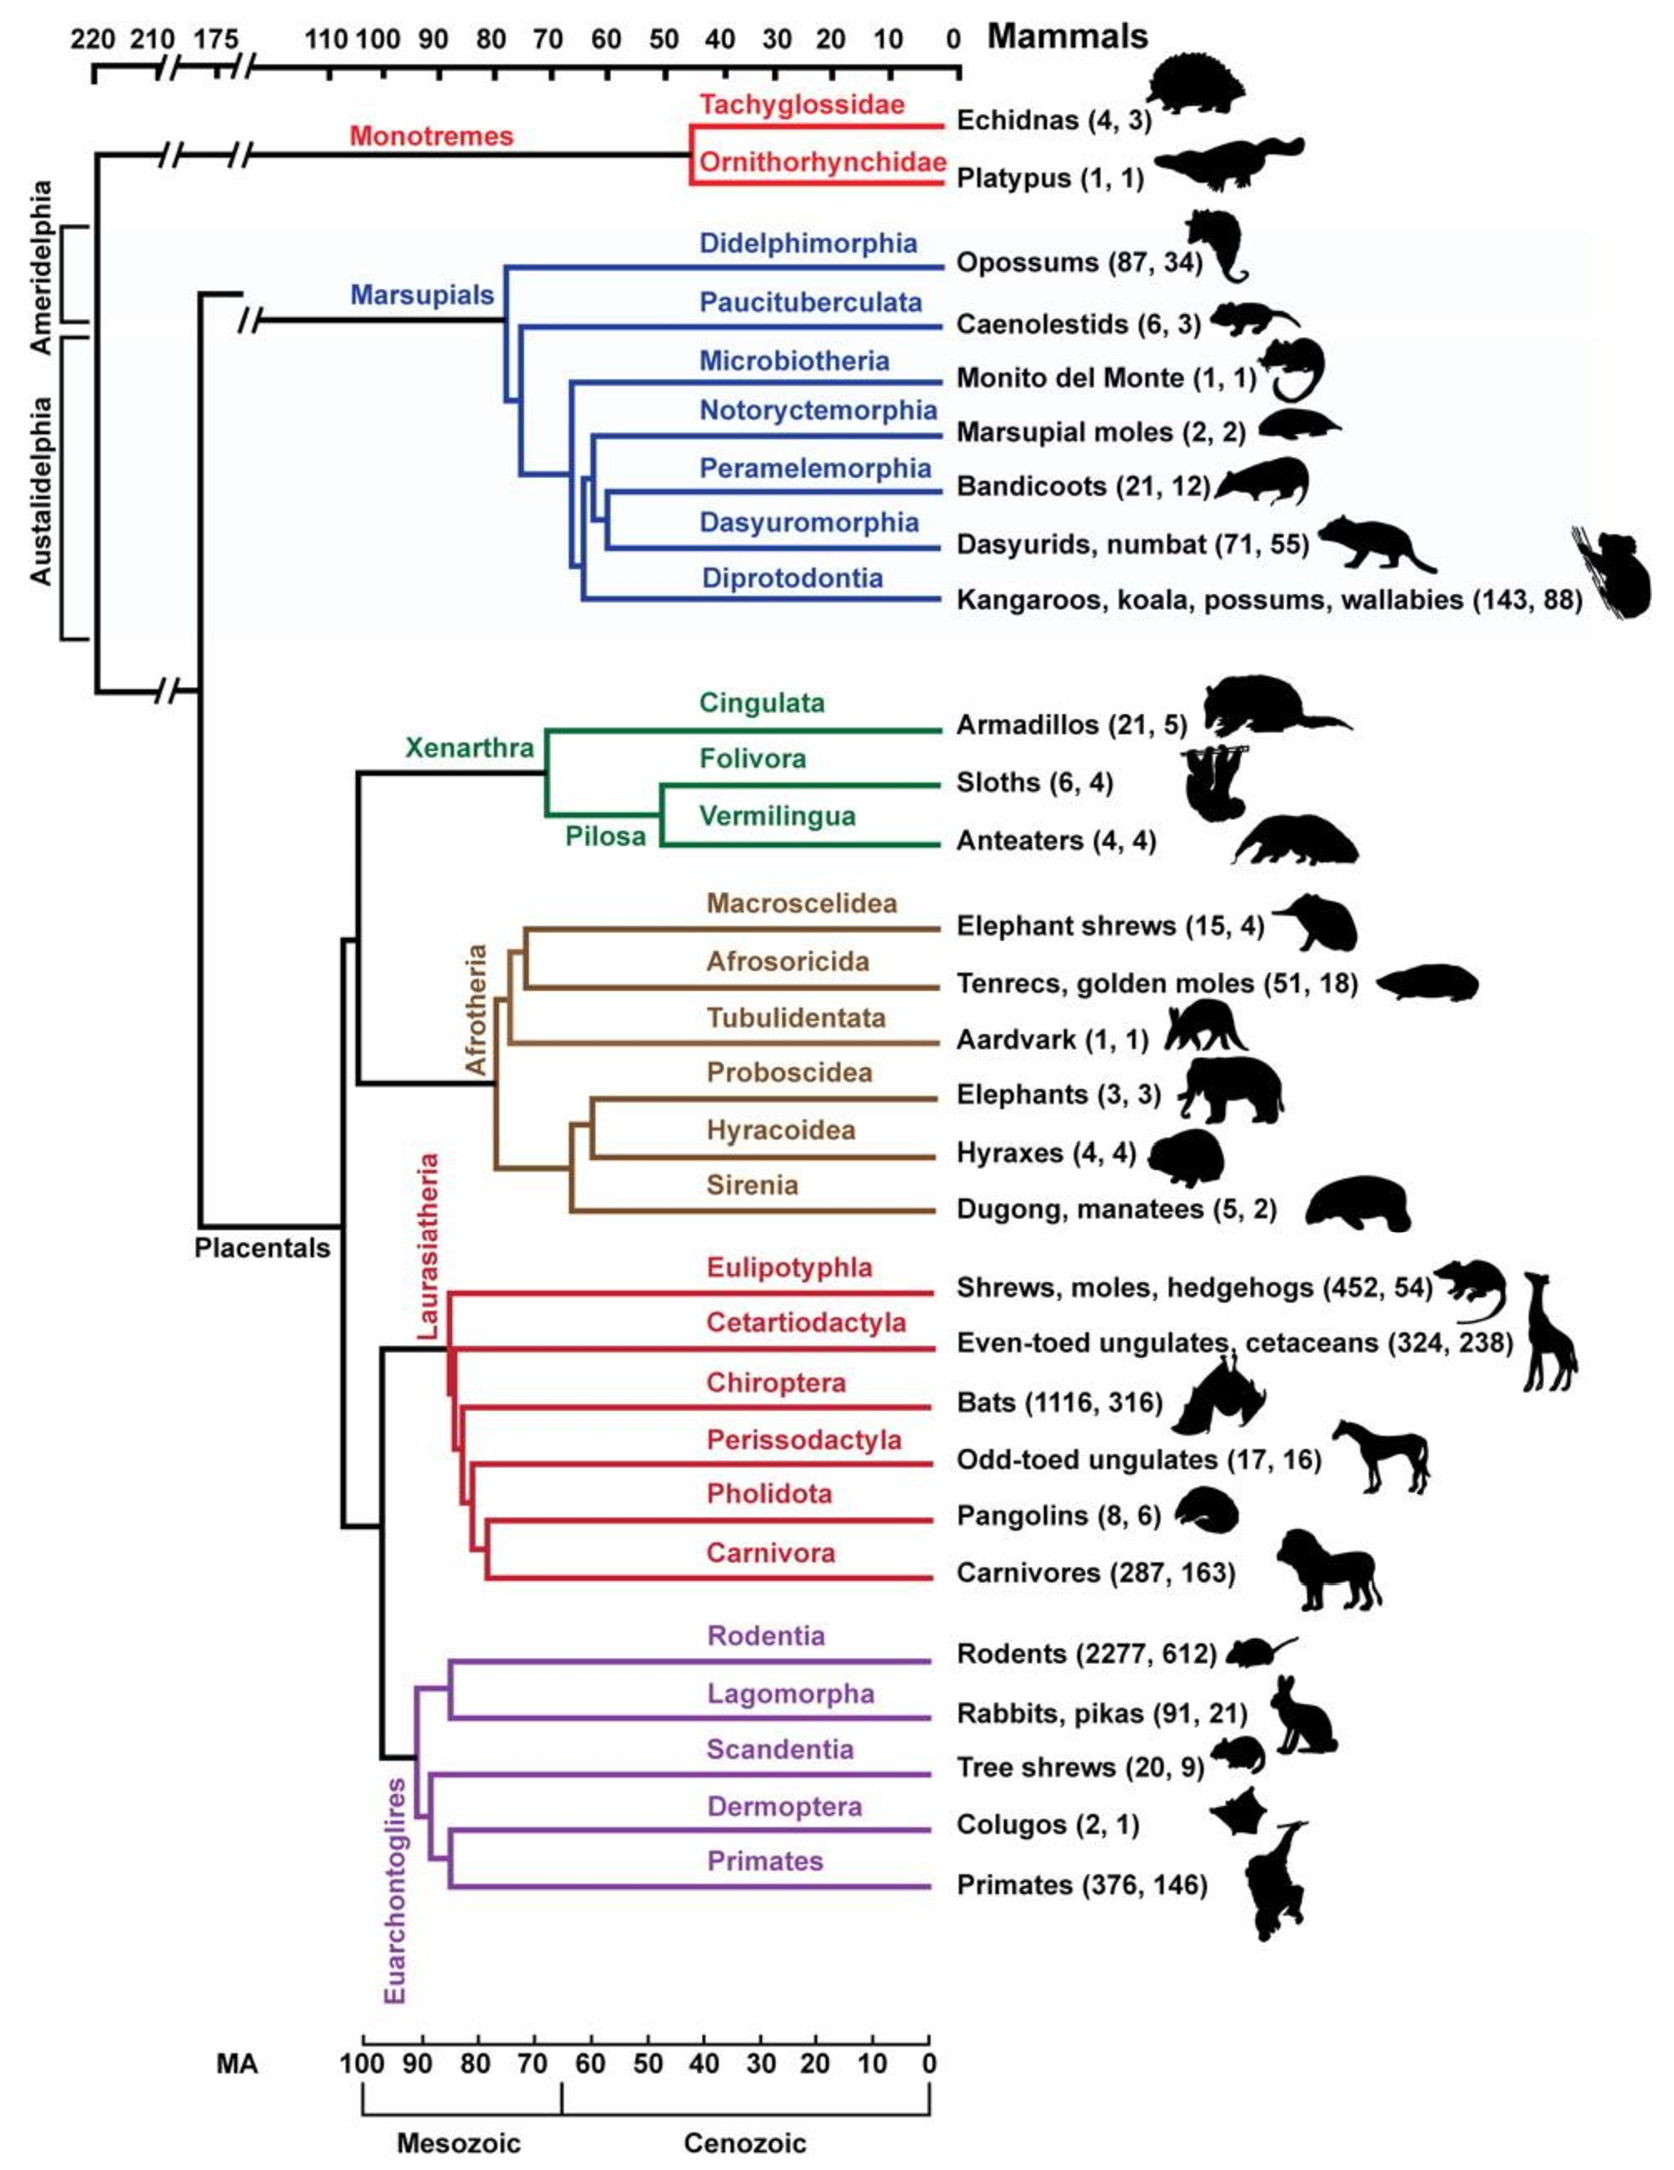
\includegraphics[scale=0.5]{Figs/mammals_10k.pdf}
\caption{A time-resolved consensus phylogeny of the major mammalian
  lineages. Topologies and dates use data from Hedges and Kumar
  \citeyearpar{Hedges2009}. Each terminal branch represents a
  mammalian family. The number of species contained in each family is
  included as the first number in parentheses after each family name
  (e.g., there are 2,227 species of rodents), while the second number
  corresponds to the number of species proposed for genome sequencing
  by \citet{Haussler2009}. Figure taken from \citet{Haussler2009}.}
\label{fig_mammals_10k}
\end{figure}

Before the K/T boundary, ancestral mammal and primate species were
likely smaller in size than they are today, as the ecological niches
for larger animals were occupied by dinosaurs
\citep{Martin2007,Smith2010}. Their diet is assumed to have been
largely insectivorous, as folivory in extant species is observed
mainly in larger mammals \citep{Smith2010} (but see \citet{Martin2007}
for an alternative perspective favoring a more folivorous primate
ancestor). After the K/T extinction event around 65 \ac{myr} ago,
mammals eventually diversified to occupy a wide range of the
ecological roles left vacant by extinct species, with many lineages
undergoing highly specialized morphological and behavioral adaptations
and the range of mammalian body sizes expanding by four orders of
magnitude \citep{Alroy1998}. A long-term trend towards larger body
sizes has been observed in many lineages; the hypothesis that this is
a general feature of mammalian evolution has been termed Cope's rule
\citep{Alroy1998}, though its universality is controversial
\citep{Finarelli2006,Monroe2010}.

The body size of mammals and their ancestors is an important
consideration in sequence analyses, as body size has been shown to
correlate with the overall rate of substitution in multicellular
eukaryotes
\citep{Mouse2002Initial,Hwang2004a,Welch2008,Galtier2009,Romiguier2010,
  Bromham2011}.  Other phenotypic features such as metabolic rate and
generation time have been similarly linked to genomic evolutionary
rates \citep{Martin1993,Nabholz2008}, but all three of these
characters are strongly cross-correlated in mammals, making it
difficult to isolate the effect of each particular variable on the
overall evolutionary rate or to identify the causative factor behind
such variation. Regardless, it is clear that extant mammals exhibit a
wide range of evolutionary rates \citep{BinindaEmonds2007b}, with
proposed explanatory factors including differences in the amount of
mutagenic free radicals associated with an animal's metabolic rate,
different rates of germ line cell divisions per year, and different
DNA repair control mechanisms \citep{Baer2007}.

\begin{figure}
\centering
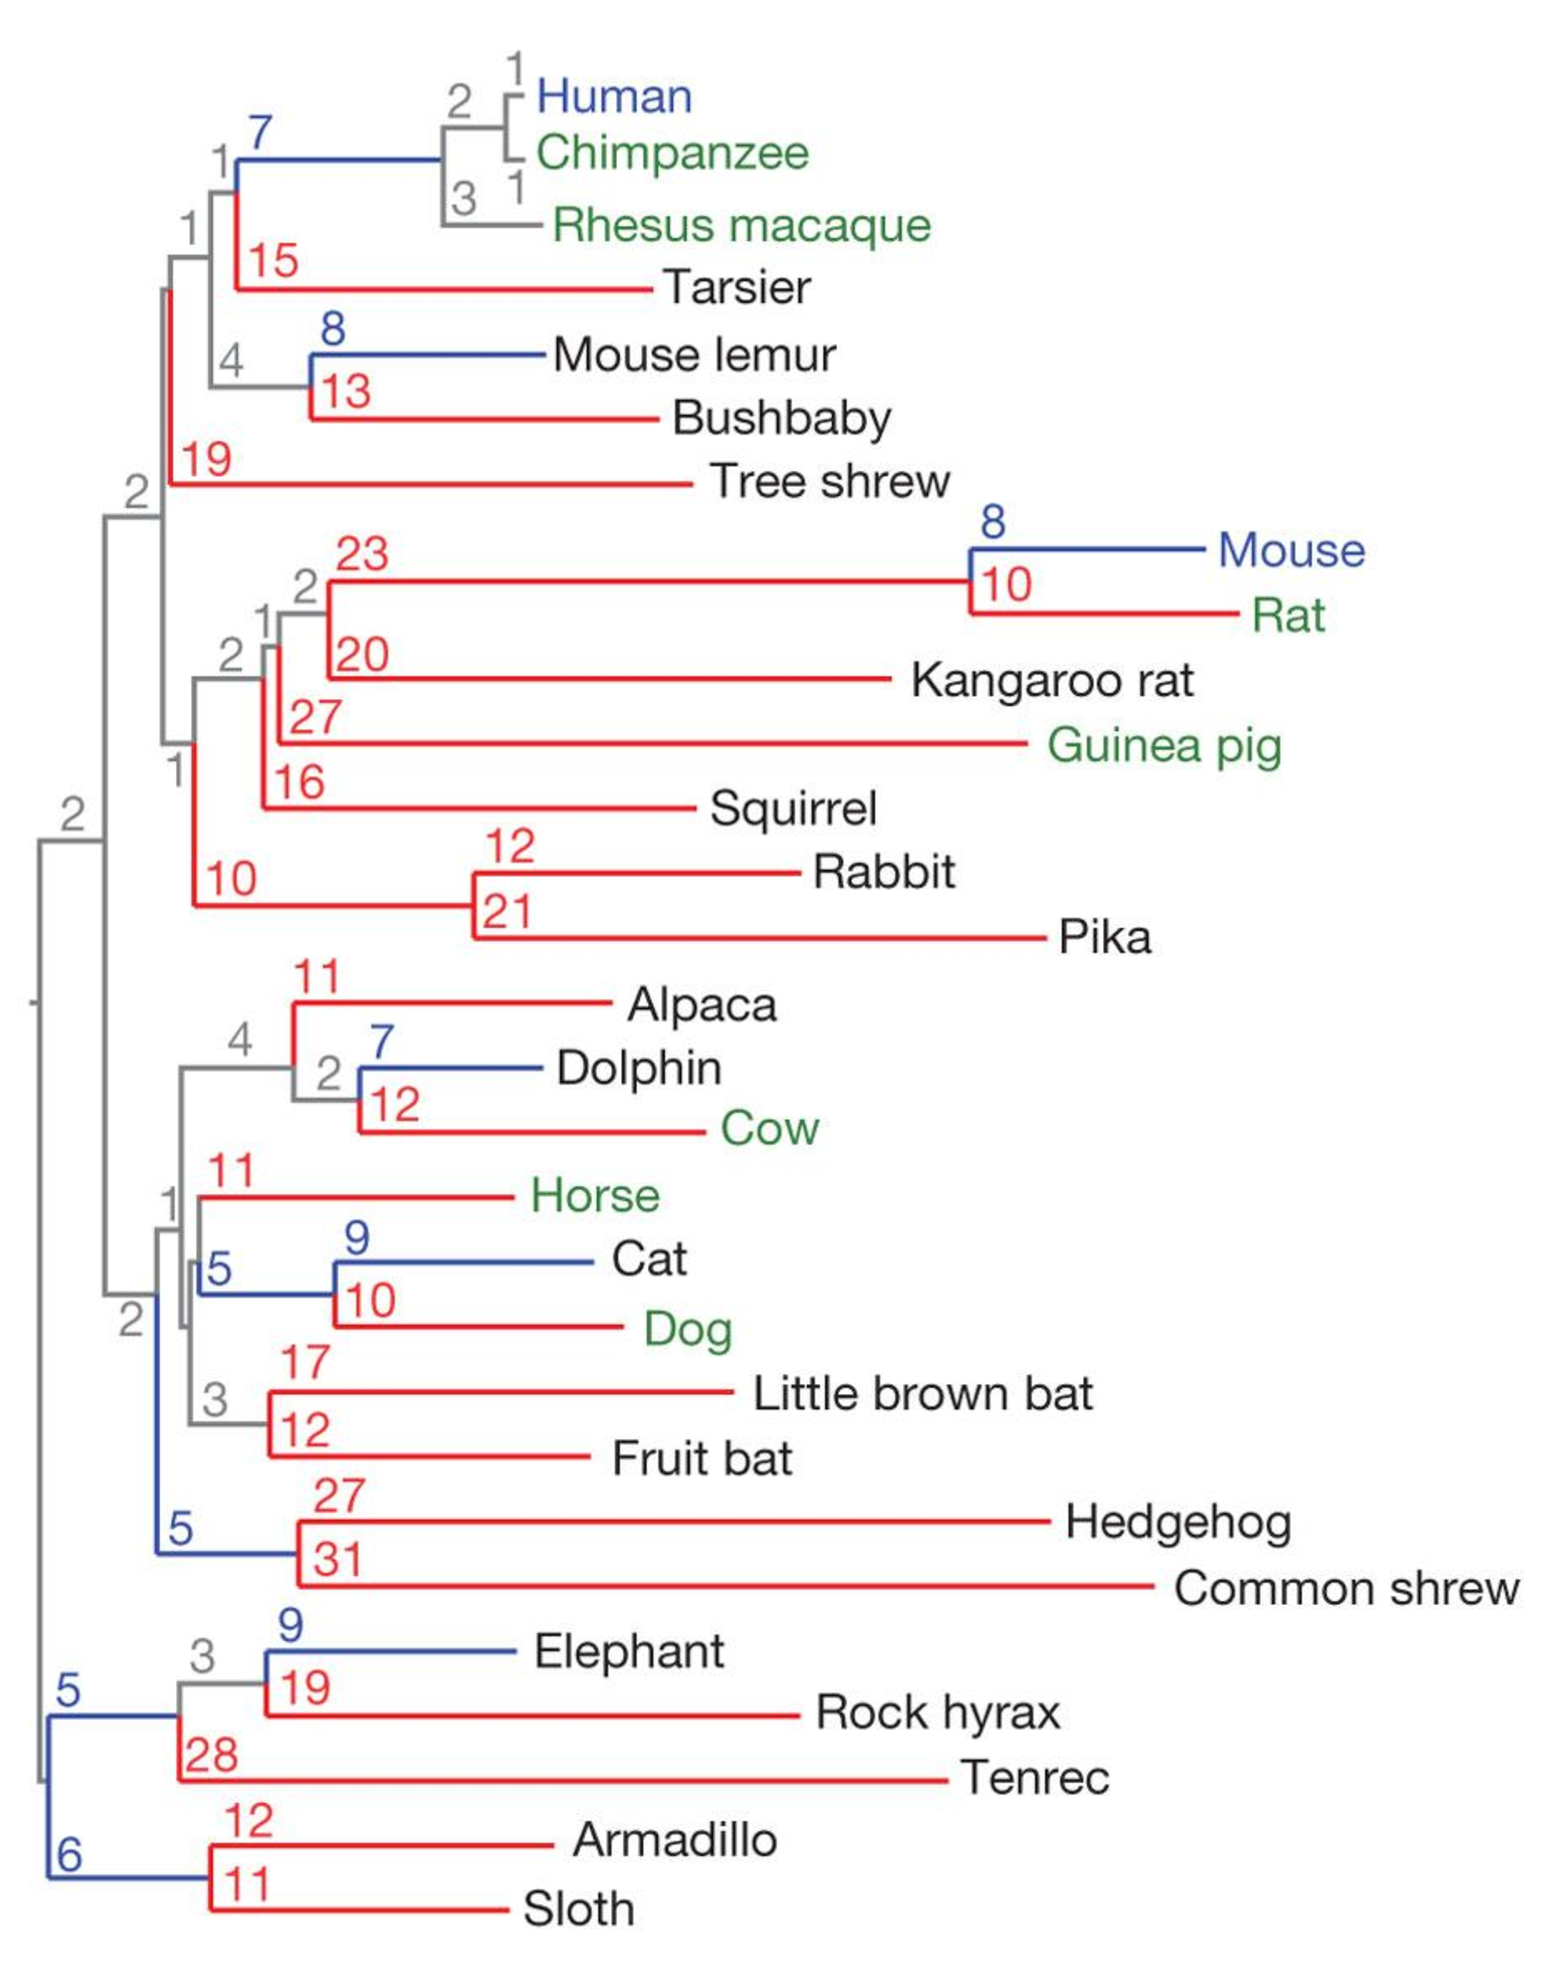
\includegraphics[scale=0.3]{Figs/mammals_29.pdf}
\caption{A phylogeny of 29 mammalian species, with branch lengths
  representing the neutral evolutionary rate estimated from
  genome-wide DNA alignments. Organisms with finished genome sequences
  are labeled in blue; those with high quality drafts are labeled in
  green; and those with low-coverage 2x assemblies are labeled in
  black. The number above each branch corresponds to the number of
  substitutions per 100bp along that branch. Branches with $\ge$10
  substitutions are colored red, branches with 5--9 substitutions are
  colored blue, and branches with $<$5 substitutions are colored
  gray. Note the increased branch lengths of most rodent species
  (e.g., mouse, rat, pika) and various small members of Laurasiatheria
  (e.g., little brown bat, hedgehog, common shrew) relative to most
  primates (e.g., human, chimpanzee). Figure taken from
  \citet{LindbladToh2011}.}
\label{fig_mammals_29}
\end{figure}

The correlation between body size and neutral evolutionary rate has an
important consequence for comparative genomic studies in mammals:
extant species groups with smaller body sizes are expected to have
experienced more DNA substitutions since their common ancestor than
larger-bodied species groups, leading to increased branch lengths
within smaller-bodied clades when branches represent the neutral
evolutionary rate (defined as the rate of evolution in genomic regions
not subject to the pressure of natural selection; the distinction
between neutrally and non-neutrally evolving sequence is covered in
more detail in Section \ref{section_evolution_models}). Figure
\ref{fig_mammals_29} shows a phylogenetic tree for 29 mammals where
branch lengths correspond to the genome-wide mean expected number of
substitutions per site within neutrally-evolving regions. This scaling
emphasizes the high observed substitution rates of most rodents and
the low rates of most hominids and some larger-bodied species from
other mammalian orders. In comparative analyses, where a larger number
of substitutions generally increases the power of a method to detect a
genomic feature or estimate an evolutionary rate (as is the case for
detecting conserved regulatory elements or positively-selected genes),
the larger branch lengths of smaller-bodied species would be expected
to result in improved power and statistical accuracy. This effect will
be especially important in Chapter~\ref{ch_mammals1} where I compare
\sw estimates of selection pressures from groups of species from
different mammalian orders. It should be noted, however, that in some
cases increased divergence levels may not result in increased
power. When sequences are extremely divergent, the accurate estimation
of distances becomes difficult and some methods may suffer as a
result; this effect is sometimes referred to as ``saturation'' of
sites.  Additionally, sequences separated by greater divergence levels
may have experienced greater numbers of independent biological
sequence insertions or deletions. These events can be difficult to
accurately reconstruct when aligning sequences, and errors in the
construction of alignments may also reduce power; this effect is
explicitly tested in Chapter \ref{ch_indels1} for the \sw detection of
positive selection.

A second biological characteristic showing significant variation
between mammals, the \ac{ne}, has important consequences for the study
of genomic regions subject to natural selection
\citep{Charlesworth2009}. \ac{ne} is a fundamental parameter in
population genetics, describing the size of an idealized population
that exhibits the same amount of dispersion of allele frequencies due
to genetic drift as the real population under study
\citep{Wright1931,Woolfit2009}. The \ac{ne} is generally smaller than
the census population size; the magnitude of this difference depends
on how strongly the assumptions of the Fisher-Wright model of an
idealized population---which include random mating, an equal sex
ratio, non-overlapping generations and a Poisson-distributed number of
offspring---are violated. As a result, many aspects of a natural
population can influence its \ac{ne}, including the census count,
breeding patterns, and geographical distribution of individuals
\citep{Caballero1994}, and studies within mammals have consistently
shown a much larger \ac{ne} for rodents than for primates and for
small versus large mammals
\citep{EyreWalker2002,Popadin2007,Halligan2010}, suggesting that
extant mammalian populations can vary significantly in this
parameter. It is beyond the scope of this thesis to provide a
comprehensive discussion of \ac{ne} and its importance within
population genetics and molecular evolution, but \citet{Woolfit2009}
and \citet{Charlesworth2009} provide focused reviews of the
subject. As it relates to this thesis, \ac{ne} can be viewed as a
measurement of the influence of genetic drift, defined as the tendency
for the frequencies of alleles within a population to change over time
due to random sampling, within a population.

The main predicted impact of \ac{ne} on the study of fixed
substitutions between species is that some slightly deleterious
mutations are more likely to become fixed within a population having a
small \ac{ne} versus a population with a large \ac{ne}. This results
from the differential influence of genetic drift: in a population with
large \ac{ne}, natural selection acts efficiently to weed out alleles
containing slightly deleterious mutations, whereas a population with
small \ac{ne} is more subject to the sampling effects of genetic drift
and is more likely to see slightly deleterious mutations reach 100\%
frequency within the population (i.e.\, become fixed). Closely tied to
this effect is the prediction of the nearly neutral thoery of
molecular evolution \citep{Kimura1985} that many mutations in
protein-coding regions are slightly deleterious and thus subject to
this dependence on \ac{ne}
\citep{Kimura1974,Kimura1985,Ohta1992}. Several empirical studies have
supported this hypothesis, showing that a different \ac{ne} leads to
different rates of protein evolution in bacteria
\citep{Moran2008,Warnecke2011}, birds \citep{Axelsson2009} and mammals
\citep{Kosiol2008,Ellegren2009} (but see \citet{Bachtrog2008} for
potentially contradictory evidence from \emph{Drosophila}). Any
analysis of comparative evolution in mammals should thus evaluated
with respect to these well-established trends; in Chapters~
\ref{ch_mammals1} and~\ref{ch_mammals2} I consider the possible
effects of \ac{ne} on the observed patterns of positive selection
within different groups of mammals, and in Chapter~\ref{ch_gorilla} I
use genome-wide \dnds ratio estimates (a fundamental measurement in
the study of protein evolution which will be introduced in Section
\ref{section_codon_models}), to compare the relative efficacy of
natural selection (and through the prediction of the nearly neutral
theory, the ancestral \ac{ne}) between our closest primate relatives
and their ancestral lineages.

Some key features of the mammalian genome itself are also worth
highlighting. Mammals contain relatively large genomes (containing
roughly 3 Gb of DNA, ranging from 2.5 to 4.5 Gb) with between 20 to 80
chromosomes \citep{Bachmann1972}. The large range in chromosome count
is likely a result of the high rate of chromosomal rearrangement in
mammals \citep{Eichler2003,Pevzner2003}. Some regions termed
``rearrangement hotspots'' show especially large amounts of
large-scale genomic shuffling within mammals, and it has been
speculated that these regions have contributed to the many
lineage-specific gene family expansions which are found in mammals
\citep{Eichler2003}. Breakpoints of mammalian chromosomal
rearrangements tend to occur near transposable elements
\citep{Zhao2009}, which are small DNA sequences capable of replicating
throughout the genome \citep{Lander2001}. Transposable elements, a
diverse class of sequence elements representing a variety of
transposition mechanisms and sequence characteristics, together
comprise roughly 45\% of DNA in the human genome and have contributed
significantly the ancient and ongoing evolution of mammalian genomes
\citep{Lander2001,Cordaux2009}.

In contrast to the rapid turnover of noncoding DNA and high rate of
genomic rearrangement observed in mammalian genomes, the
protein-coding gene complement appears to be less variable. Initial
estimates of roughly 30,000 protein-coding gene
\citep{Lander2001,Mouse2002Initial} in the human and mouse genomes
have been lowered based on accumulating functional and phylogenetic
evidence to roughly 21,000 genes \citep{Macaque2007}; the most recent
gene annotations from \ens \citep{Flicek2011} contain 20,599 human and
21,873 mouse ``known'' protein-coding genes. A majority of these genes
are shared between all mammals: human and mouse share an estimated
80\% of genes in a ``one-to-one'' fashion, meaning no apparent gene
duplications or deletions occurred since the common ancestor
\citep{Mouse2002Initial}, and a wider group of mammals including
platypus show detectable orthologs (including genes with duplications
or deletions in one or more lineages) in 82\% of genes
\citep{Warren2008b}. Despite the relative consistency of the mammalian
protein-coding catalogue, features such as alternative splicing and
domain concatenations have been identified as potential contributors
to mammalian phenotypic complexity and diversity \citep{Lander2001}.

In any study of vertebrate protein-coding genes, the \ac{2rgd}
hypothesis looms large. Originally proposed by \citet{Ohno1970}, the
\ac{2rgd} hypothesis suggests that two polyploidization events occurred
during the early evolution of the vertebrate common ancestor,
explaining the observation that vertebrates often have up to four
homologs of invertebrate genes \citep{Hokamp2003}. For three decades
the veracity of the \ac{2rgd} hypothesis was hotly debated
\citep{McLysaght2002,Dehal2005}, but analyses based on comparisons
between whole-genome sequences of several fish and basal chordates
have repeatedly confirmed its predictions
\citep{Kasahara2007,Putnam2008b}. In addition to having interesting
implications for the evolution of the immune system and of
morphological diversity within vertebrates
\citep{Hughes1997,Hoffmann1999,Peer2009b}, the existence of ancient
genomic duplications can cause problems in the inference of homology
relationships between genes. Many of these aspects will be considered
in more detail in Chapter~\ref{ch_orthologs} when a set of mammalian
orthologs suitable for evolutionary analysis is identified.

\section{Models of sequence evolution}
\label{section_evolution_models}

The previous section described the major genomic and evolutionary
features of mammalian species. It is important to note that the
majority of those well-established observations were made by fitting
mathematical models of sequence evolution to comparative genomics
data, which is now a standard analytical approach. This section
briefly introduces the methods and models of evolutionary analysis
which will be applied throughout the remaining chapters.

As the hereditary material of all free-living organisms, DNA
represents a record of the history of life on earth. When an
individual gives rise to offspring, special segments of DNA are
replicated and passed on to all its descendants; importantly, the
processes of DNA replication and repair are imperfect
\citep{Arnheim2009} and the resulting errors, called mutations, can be
passed on to successive generations if they occur in germline
cells. In addition to being a major source of the variation between
individuals invoked in Darwin's theory of natural selection
\citep{Darwin1859a}, mutations in DNA leave a molecular record of
evolutionary relationships and of the passage of time. Mutations arise
in individuals, are passed on to descendants through DNA replication,
and subsequently increase or decrease in their frequency within a
population over time due to the survival or death of individuals
containing that mutation. Sometimes a mutation reaches 100\% frequency
within the population, at which point it has become ``fixed'', or
shared between all individuals of a population.

The fixation of mutations within independently evolving populations
produces observed differences in the DNA sequences of different
species at homologous locations. The most commonly observed type of
fixed DNA mutation is where one nucleotide base is substituted for
another; these differences, called point mutations or substitutions,
can be reasonably modeled using phylogenetic trees and Markov models
of sequence evolution \citep{Yang2006}. Other common mutation types,
however, are less amenable to modeling. Short sequence insertions or
deletions, which occur roughly 10\% as frequently as base
substitutions, result in either the loss of genetic information from a
lineage (in the case of a deletion) or the incorporation of genetic
information which does not share a simple common ancestor with other
lineages (in the case of an insertion). As a result, sequence
insertions and deletions are not as easily modeled as base
substitutions. The presence of many insertions and deletions within
related sequences can make the assignment of homology between sequence
positions---a process referred to as alignment---difficult. This
thesis explores some aspects of alignment error on downstream
evolutionary analyses, especially in Chapter \ref{ch_indels1}. Other
possible types of mutations, including chromosomal rearrangements,
large-scale duplications and deletions of genomic regions, and
horizontal gene transfer, are also important in genome evolution but
will not be studied extensively in this thesis.

The rest of this section will introduce the many mathematical models
constructed to describe the accumulation of point mutations over
time. The earliest observations that biological sequences tend to
change randomly over time were made from sequences of proteins, the
main molecules of cellular machinery comprised of amino acid units
whose arrangement is encoded in the DNA sequences of exons within
genes. In the early 1960s, Zuckerkandl and Pauling were analyzing the
amino acid sequences of hemoglobin genes from various species. They
noted that the number of changes between sequences from different
species corresponded well with the evolutionary distance those species
based on fossil evidence; this led them to hypothesize that evolution
at a molecular level may occur at a largely constant rate
\citep{Zuckerkandl1962,Morgan1998}. Zuckerkandl and Pauling continued
to explore the implications and applications of this ``molecular
evolutionary clock'' hypothesis, using hemoglobin and cytochrome C
sequences to estimate the date of human-gorilla divergence (at 11
million years) and to infer the protein sequences of mammalian
ancestors \citep{Zuckerkandl1965}. A wide variety of evolutionary
models has subsequently been developed to describe observed patterns
of amino acid and DNA substitutions. As this thesis is concerned
largely with the application of such methods, I will only briefly
summarize the key features of the more popular evolutionary models;
\citet{Yang2006} provides a comprehensive mathematical treatment of
the main models used in practice.

The simplest Markov model for DNA substitution, proposed by
\citet{Jukes1969a}, assumes that every nucleotide has the same rate of
changing into any other nucleotide. Although the assumption of equal
rates is a reasonable starting point for modeling a random process,
the mutation of a DNA base pair is a biochemical process (or rather, a
set of potentially many unobserved biochemical processes which all
produce the same class of observable result), making the existence of
biases towards or against certain types of mutations highly
plausible. This was quickly discovered to be the case: analysis of the
ever-increasing number of available biological DNA sequences showed
that in most datasets \emph{transitions}, defined as substitutions
between two pyrimidine nucleotides (i.e., T$\to$C or C$\to$T) or
between two purine nucleotides (i.e., A$\to$G or G$\to$A), are more
common than \emph{transversions}, defined as substitutions from a
purine to a pyrimidine or vice-versa. \citet{Kimura1980} thus proposed
a more complex model, called K80 or Kimura's two-parameter model,
which accounted for this bias. Specifically, K80 extends JC69 by
incorporating an additional parameter, $\kappa$, referred to as the
transition/transversion ratio, representing the ratio of the rate of
transition substitutions to the rate of transversion
substitutions. When $\kappa$ is greater than one, transitions occur at
a higher rate than transversions, providing a better fit to most
biological datasets \citep{Brown1982}. The $\kappa$ parameter of K80 a
prototypical example of the parametric approach to building
evolutionary models, whereby a parameter is introduced into the model
which allows for a commonly-violated assumption of the simpler model
to be relaxed. Note that the value of the parameter is not specified
in the model; rather, it must be provided or estimated from the data
on a case-by-case basis, usually by \ac{ml} estimation
\citep{Whelan2001}.

Several nucleotide models were subsequently described which relax
various further assumptions of the JC69 and K80 models
\citep{Whelan2001,Yang2006}. One especially unrealistic feature of K80
is its symmetric nature (meaning that the rate of substitution from
one nucleotide to another is the same as the rate of the reverse
substitution, e.g. G$\to$C = C$\to$G). A symmetric DNA Markov chain
yields equal nucleotide frequencies when the substitution process
reaches equilibrium, meaning that any starting DNA sequence, if left
to evolve long enough under such a process, will end up with equal
nucleotide frequencies. In reality, many biological sequences contain
highly unequal nucleotide frequencies (owing to a variety of possible
selective or mutational biases), making it inappropriate to assume an
equal base composition \citep{Yang2006}. Thus, models such as FEL
\citep{Felsenstein1981a}, HKY \citep{Hasegawa1985} and TN93
\citep{Tamura1993} were developed to allow for various combinations of
unequal base frequencies and unequal transition/transversion
ratios. The most general reversible nucleotide model, REV, includes
three parameters to describe the equilibrium nucleotide frequencies
(where the frequency of the fourth nucleotide is determined by the
requirement that all frequencies must sum to 1) and six rate
parameters, one for each possible pair of substitutions
\citep{Tavare1986}.

In contrast to the primarily parametric DNA models, evolutionary
models for amino acids have generally been estimated empirically
\citep{Whelan2001}. The JTT \citep{Jones1992} and Dayhoff
\citep{Dayhoff1978} amino acid models were estimated using
parsimony-based counting methods, using substitutions inferred from
closely-related sequences to fill the entries of the 20x20 amino acid
substitution matrix; these counts were then used to estimate
reversible Markov substitution models. More recently, empirical amino
acid models were estimated using \ac{ml} methods, which improved upon
a number of methodological deficiencies of the parsimony approach
\citep{Adachi1996,Whelan2001b,Le2008}.

At this point it should be pointed out that a few important
assumptions are shared by all of the models already described, namely
that all sites within an alignment are (a) evolving independently of
one another, (b) evolving under the same evolutionary process and at
the same evolutionary rate, and (c) related by the same underlying
phylogenetic tree. These assumptions are clearly violated in many real
datasets, so I will briefly review the development of models which
relax them to various degrees.

Independence between sites is generally a difficult assumption to
relax for computational reasons \citep{Kosiol2006c}, but the
hypermutability of CpG dinucleotides within mammalian genomes (where
CpG denotes a C nucleotide followed by a G nucleotide, the ``p''
representing the phosphodiester bond separating nucleotides on the
same strand of a DNA molecule) has provided strong impetus to
incorporate at least a dinucleotide context into models for estimating
nucleotide substitution rates from large mammalian alignments
\citep{Blake1992,Hwang2004a,Siepel2004a}. CpG hypermutability results
from the methylation and subsequent deamination of the cytosine
nucleotide at CpG sites in most mammalian genomic DNA. Although all
cytosine nucleotides are prone to deamination (whether methylated or
not), cytosine deamination produces uracil, which is removed from DNA
strands by the enzyme uracil glycosylase, allowing for DNA repair
mechanisms to replace the original cytosine. On the other hand, the
deamination of 5-methylcytosine produces thymidine, which is not
efficiently repaired and results in frequent C$\to$T transitions
\citep{Ehrlich1982,Hwang2004a}. Context-dependent substitution models
have shown that CpG mutations are by far the dominant form of mutation
in mammalian genomes, and such models have also been essential for
studying the evolution of GC content and mammalian isochores
\citep{Duret2006,Duret2008}.

The assumption of a homogeneous evolutionary process acting across all
alignment sites is often violated in real datasets of all sequence
types \citep{Yang2006,Whelan2008}, and the development of methods
allowing for this assumption to be relaxed in the analysis of various
types of sequences has long been an area of productive research. Most
studies have focused on across-site variation of a single parameter
such as the evolutionary rate
\citep{Uzzell1971,Yang1994c,Yang1996,Nielsen1998}, but more complex
types of heterogeneity, such as heterogeneity in the entire rate
matrix which describes the evolutionary process, have also been
explored \citep{Lartillot2004} . The approach generally taken for
variation of a single parameter is to describe the rate (or whichever
parameter is being modeled as varying across sites) for each site as a
random draw from a statistical distribution. In this way, the
mathematically convenient assumption of independence between sites is
upheld while sites are allowed to vary according to the parameter of
interest. The gamma distribution is commonly used for this purpose, as
it contains only one parameter if the mean rate is normalized to
1. This parameter, $\alpha$, is typically estimated from the data and
has a very clear interpretation: low values of $\alpha$ reflect an
L-shaped gamma distribution with a large amount of rate variation,
while high values of $\alpha$ reflect a bell-shaped distribution where
most sites evolve near to the average rate.

The final assumption of a single phylogenetic tree relating all sites
within a sequence has been less studied. Simulations have been used to
evaluate the potential impact of recombination
\citep{Anisimova2003,Shriner2003} and gene conversion
\citep{Casola2009} on the use of evolutionary codon models (introduced
in the next section) to detect positive selection, finding that
moderate levels of false positives occur when the assumption of a
single tree is violated. Simulations have also been used to estimate
the impact of recombination on reconstruction of ancestral sequences
\citep{Busto2010} and phylogeny inference \citep{Schierup2000}. In
virus genetics where recombination is commonly encountered, methods
have been developed to automate the identification and handling of
recombination events in evolutionary analyses
\citep{Grassly1997,Pond2006}. Additionally, in comparative genomic
analyses of closely-related species, the tree relating the species'
sequences may vary across the genome due to \ac{ils}. This is
encountered in the analysis of great ape genes presented in Chapter
\ref{ch_gorilla}, where a simple filtering scheme was used to remove
sites potentially subject to \ac{ils}.

\section{Detecting purifying and positive selection in proteins}
\label{section_codon_models}

Proteins are functionally active as folded, structured amino acid
molecules, but the genes which encode them replicate and mutate and
evolve as DNA molecules. The connection between DNA and protein is
mediated by the genetic code, which describes how non-overlapping
codons, or triplets of nucleotides within the coding sequence of a
protein-coding gene, are translated by the ribosome and tRNA molecules
into polymers of the 20 common amino acids. Since there are $4^3=64$
possible codons and only 20 amino acids, the genetic code is
degenerate (i.e., multiple codons are translated into the same amino
acid). This degeneracy is concentrated in the third codon position,
with many codons differing by only their third nucleotide coding for
the same amino acid, but some degeneracy also exists in the first
position. No codons differing by their second nucleotide encode the
same amino acid. Only two amino acids, methionine and tryptophan, are
encoded by just one codon, and three codons are stop codons used
uniquely to signal the end of the peptide chain.

The degeneracy of the genetic code causes some changes on the DNA
level to be \syn, meaning they result in no change to the encoded
amino acid sequence, while others are \nsyn, meaning they result in an
altered protein sequence. The decoupled nature of the process of DNA
mutation, which is presumably ``unaware'' of the genetic code and
affects all nucleotides equally, and the process of natural selection,
which acts on phenotypes typically (but not exclusively) affected by
protein structure, suggests that a comparison of rates of \nsyn and
\syn substitution would allow the influence of natural selection
acting on a protein to be detected while inherently correcting for the
neutral mutation rate. Indeed, the potential of this approach was
noted by various researchers as soon as large-scale DNA sequencing
became practical \citep{Kimura1977,Jukes1979}, and the comparison of
the rate of \nsyn substitution ($d$N) and the rate of \syn
substitution ($d$S) has been a cornerstone of the evolutionary
analysis of proteins since then \citep{Yang2006}. Various techniques
were historically used to estimate \dn and \ds \citep{Yang2000c}, but
most modern software is based on one of the two parametric Markov
models for coding sequence evolution independently proposed by
\citet{Goldman1994a} and \citet{Muse1994} or, when an empirical codon
model is desirable, a version of the model estimated by
\citet{Kosiol2007}.

Although the two parametric codon models differ in the details of how
nucleotide and codon frequencies are handled
\citep{Yang2000c,Bierne2003a}, they are similar in that each
incorporates a selection parameter $\omega$, representing the ratio of
\dn and \ds, into a Markov model of coding sequence evolution. The
$\omega$ parameter has a simple interpretation, namely that it
measures the ``the net effect of selection at the protein level''
\citep{Yang2000CodonSubstitution}. When $\omega=1$, natural selection
acts neither for nor against protein change, and the sequence is said
to be evolving neutrally; when $\omega<1$, selection acts to conserve
the protein sequence, exerting a so-called purifying selective
pressure; when $\omega>1$, selection acts to change the protein
sequence, exerting a so-called positive selective pressure. Within the
context of population genetics, the $\omega$ parameter can be linked
to $s$, the selective coefficient of an allele segregating in the
population \citep{Nielsen2003,Nielsen2005b,Kryazhimskiy2008}, with
$\omega>1$ corresponding to $s>0$ and $\omega<1$ corresponding to
$s<0$. This interpretation involves many assumptions, however, and has
found little practical use \citep{Nielsen2003,Nielsen2005b}.

For either of these Markov codon models (as well as for the simpler
models of DNA and protein evolution described earlier), parameters
(here including $\omega$, $\kappa$, and branch lengths for the model
of \citet{Goldman1994a}) can be numerically optimized for a given
alignment and phylogeny by maximum likelihood using Felsenstein's
pruning algorithm \citep{Felsenstein1981a,Goldman1994a,Yang2000c}. In
their initial description of the model, \citet{Goldman1994a} presented
an example modification to the model which allowed for heterogeneous
substitution rates across sites using an approach similar to that
described above for nucleotide models. Much subsequent work has been
focused on developing models allowing for variation of $\omega$ across
sites in the alignment
\citep{Nielsen1998,Yang2000CodonSubstitution,Yang2002,
  Wong2004,Yang2005Bayes,Massingham2005}, between branches in the tree
\citep{Yang1998a}, or both \citep{Yang2002b,Zhang2005}.  A detailed
account of these developments will not be presented here
(\citet{Anisimova2009} provide a comprehensive review of the
state-of-the-art in probabilistic codon models), but three codon-based
models in particular are used extensively throughout this thesis to
examine patterns of natural selection within mammalian proteins: the
branch model and sites models implemented in the \ac{paml} program by
Ziheng Yang \citep{Yang2007} and the \ac{slr} method implemented
in the \ac{slr} program by Tim Massingham \citep{Massingham2005}. Each
of these models is introduced in more detail below.

\subsection{Branch and sites models in PAML}

For a long time, the $\omega$ ratio was almost always calculated as an
average value across an entire protein \citep{Sharp1997}. Functional
and structural constraints within a protein sequence might dominate
the gene-averaged signal of evolutionary constraint, however, even if
positive selection has acted on some portion of the protein. In some
cases, such as when the amount of computational power or data
available is limited, averaging $\omega$ across sites is a reasonable
compromise, but as computer and sequencing technologies rapidly
developed in the late 1990s, that compromise was becoming less
necessary and whole-gene estimates less justifiable. Whole-gene
$\omega$ estimates were shown to lack power \citep{Endo1996}, and
although ad-hoc analyses of $\omega$ within specific regions of proteins
were more sensitive \citep{Hughes1988}, they were limited to cases
where prior knowledge of the tertiary or domain structure of a protein
could be used to identify subsets of the protein for analysis.

As a statistically rigorous alternative, Ziheng Yang and collaborators
adopted a so-called ``random sites'' approach to modeling variation of
the $\omega$ ratio across sites for the PAML software. This
implementation typically favored modeling $\omega$ variation with a
gamma or beta distribution, discretized into a predefined number of
site classes for computational efficiency. To identify positive
selection with statistical justification, a variety of \acp{lrt} were
developed.

The \ac{lrt} is a widely-used statistical technique which tests the
goodness of fit between two models. Before returning to a description
of the \acp{lrt} designed for detecting positive selection with
variation of $\omega$ across sites, the likelihood function and the
\ac{lrt} will be briefly introduced. Given a statistical model $H$ and
a vector of unknown parameters $\Theta$, the likelihood function $L$
describes the probability of observing a given dataset $X$ as a
function of the parameters, $L(\Theta;X)=Prob(X|\Theta)$. The \ac{mle}
of the parameter vector $\hat{\Theta}$ is the set of parameters which
maximizes the likelihood of the observed data $X$. Since likelihood
values can be extremely small, the log-likelihood function
$\ell=ln[L(\Theta;X)]$ is often preferred. The \ac{lrt} statistic
$2\Delta$ compares the goodness of fit of two different models,
$H_{0}$ and $H_{1}$, with parameter vectors $\Theta_{0}$ and
$\Theta_{1}$ each containing $n_{0}$ and $n_{1}$ parameters. With
parameters set to their \acp{mle}, the maximum log-likelihood values
for $H_{0}$ and $H_{1}$ are defined as
$\ell_{0}=\ell(\hat{\Theta_{0}})$ and
$\ell_{1}=\ell(\hat{\Theta_{1}})$, respectively, and the \ac{lrt}
statistic $2\Delta$ for comparing goodness of fit is simply twice the
difference of maximum log-likelihood values, $2\Delta = 2[\ell_{1} -
  \ell_{0}]$. When $H_{0}$ is nested within $H_{1}$ (e.g., when
$H_{0}$ is equivalent to $H_{1}$ with a single parameter held at a
constant value, leading to $n_{1}-n_{0}=1$) then $2\Delta$ is asymptotically distributed as
$\chi^{2}_{n_{1}-n_{0}}$ when the null model $H_{0}$ is true. By
comparing the \ac{lrt} statistic to the critical value of the
appropriate $\chi^2$ distribution, the hypothesis that a more complex
model better describes the observed data can be tested
\citep{Wilks1938,Yang2006}. When comparing non-nested models or nested
models where a parameter is fixed at the boundary of possible values,
the $\chi^2$ approximation does not hold; in some cases a mixture of
distributions may be appropriate \citep{Whelan1999}, but in other
cases parametric simulations are needed to estimate the null
distribution of the \ac{lrt} statistic \citep{Goldman1993a}.

In the context of detecting positive selection, the most effective
\acp{lrt} typically compare a model allowing for some variation of
$\omega$, but not allowing $\omega>1$, to a more complex model which
additionally allows for $\omega>1$ (the former model being nested
within the latter). \citet{Nielsen1998} initially proposed a few
simple \acp{lrt} for detecting positive selection; these were further
expanded and evaluated by \citet{Yang2000CodonSubstitution}, and
\citet{Anisimova2001} performed extensive simulations assessing the
power and accuracy of these tests. The current release of PAML
recommends two \acp{lrt} for detecting positive selection acting at a
subset of sites within genes: \mbox{M2a--M1a} and \mbox{M8--M7} (see
Table 1 in \citet{Wong2004} for a complete description of each
model). PAML also implements a method for identifying which individual
sites show strong evidence for positive selection. This method, called
the Bayes Empirical Bayes method and described in
\citet{Yang2005Bayes}, calculates for each site an approximate
posterior probability that it has been subject to positive
selection. I evaluate the power of this method for detecting \sw
positive selection in Chapter \ref{ch_indels1}.

Codon models relaxing the assumption of a constant $\omega$ throughout
the branches of the tree, but not across sites, were also developed
and implemented in PAML \citep{Yang1998,Yang1998a}. Although these
models have received less attention and use than the branch-site
models, which allow $\omega$ to vary across both sites and branches
\citep{Zhang2005}, they may be useful when branch lengths are small
and parameter estimation under the complex branch-site models is
difficult, or when variation of $\omega$ across sites is not of
interest. These models are used in Chapter \ref{ch_gorilla} to
construct a series of \acp{lrt} for detecting accelerated evolution
along specific branches of the great ape tree.

\subsection{The Sitewise Likelihood Ratio method}

In contrast to PAML's approach to site-specific evolutionary analysis,
where a \ac{lrt} for positive selection within a gene is first
performed and, subject to a significant \ac{lrt} result, \sw posterior
probabilities for positive selection are then inferred, the \ac{slr}
method \citep{Massingham2005} was specifically designed for the
sitewise estimation of purifying and positive selection. \ac{slr} is
based on a Markov model of codon evolution similar to that of
\citet{Goldman1994a}. No assumptions are made regarding the
distribution of $\omega$ ratios within the alignment; instead, the
value of $\omega$ is considered to be an independent parameter at each
site, $\omega_{i}$ for site $i$. The idealized \sw \ac{lrt} for
positive selection then compares the log-likelihood value of a null
model where $\omega_{i}=1$ to a model where $\omega_{i}$ is optimized
to its \ac{mle}. As the estimation of model parameters and calculation
of likelihood values to perform an exact \ac{lrt} at each site would
involve an expensive high-dimensional optimization, \ac{slr} uses two
approximations which greatly reduce the computational complexity:
first, parameters common to all sites (including branch lengths,
$\kappa$ and the equilibrium codon frequencies) are estimated under
the M0 model \citep{Yang2000CodonSubstitution} with one $\omega$ for
all sites instead of the more parameter-rich true null model, and
second, the \sw $\omega$ parameter is estimated independently at each
site under the simplifying assumption that each site's contribution to
the common parameters is minimal \citep{Massingham2005}. In practical
terms, \ac{slr} uses the common parameters and the alignment data at
each alignment site to calculate a sitewise statistic for non-neutral
evolution. This statistic is based on a likelihood-ratio test where
the null model corresponds to neutral evolution by holding the
$\omega$ parameter fixed at 1 and the alternative model uses the
\ac{mle} of $\omega$. The raw \ac{slr} statistic measures the strength
of evidence for non-neutral evolution at each site, and the observed
statistic can be compared to its theoretical distribution under the
null model, \chisq, to identify sites with evidence for purifying or
positive selection at a desired significance threshold. Simulations
performed by \citet{Massingham2005} showed \ac{slr} to perform as well
as or better than PAML's random sites models at detecting positive
selection within genes under some conditions; Chapter \ref{ch_indels1}
provides further assessment of the power of the \ac{slr} method to
detect \sw positive selection under a wide range of conditions, and in
Chapters \ref{ch_mammals1} and \ref{ch_mammals2} I apply \ac{slr} on a
large scale to analyze genome-wide patterns of \sw positive selection
in mammals.

\subsection{Alignment and selection analyses}

\bresp{Alignment}[Won't go into detail about methods for alignment,
  but discussion of dealing with *uncertainty*, esp. wrt selection, is needed.]

[Alignment can be ambiguous, and computationally intractable for optimal solutions]

[For ambiguity, statistical approach has often been taken. Involves
  explicit model of insertion and deletion, sampling over large
  population of suboptimal alignments, or weighting downstream estimates based on alignment probability]

[Explain why I didn't use any of these super-cool approaches here:
  computational issues, prevalence of non-indel versus indel errors,
  difficulty of directly incorporating selection estimates into
  alignment uncertainty]

\eresp{Alignment}

\section{Outline of the thesis}

This thesis describes three largely independent studies centered
around the theme of using codon models to analyze patterns of
selective constraint in mammalian genomes.

Chapter \ref{ch_indels1} describes a simulation study I conducted to
evaluate the impact of alignment error on detecting \sw positive
selection. The widespread adoption of powerful methods for sequence
analysis has been somewhat hampered by a lack of understanding of the
limitations of, and sources of error inherent within, those
methods. Without such knowledge, researchers could either avoid using
such methods for fear of producing misleading results, or blindly
apply such methods without regard for possible errors. Both paths have
been taken by others with respect to the issue of alignment error in
detecting positive selection
\citep{Thompson1994,Bakewell2007,Studer2008,MarkovaRaina2011}. As a
first step towards an improved understanding of alignment error and
its impact on downstream evolutionary analyses, I performed a thorough
examination of the impact of alignment error by comparing different
aligners, trees, and methods for detecting positive selection. This
work has been recently published \citep{Jordan2011} and is presented
in Chapter \ref{ch_indels1} largely unmodified from its published
form.

With whole-genome sequences quickly accruing in the databases at an
ever-increasing pace, I devoted a large part of my research effort
towards applying evolutionary codon models on a large scale to
mammalian and primate genomes. The rest of the thesis reflects this
focus, presenting two major empirical analyses. Chapters
\ref{ch_orthologs}, \ref{ch_mammals1} and \ref{ch_mammals2} describe
in three sections a genome-wide analysis of \sw selective pressures in
mammals that was performed in collaboration with the \acf{mgp}; a more
detailed description of the \acp{mgp} and my involvement in the
analysis is provided in the introduction to Chapter
\ref{ch_orthologs}. A highly summarized and edited version of the
results of this analyses was recently published
\citep{LindbladToh2011}, but the version presented here differs in
that a more recent dataset was used and the methods and results are
described in considerably more detail. Particular attention was paid
to identifying (and in some cases ameliorating) possible sources of
error and to comparing the current results with those from previous
similar studies in the literature.

Chapter \ref{ch_gorilla} presents a more detailed survey of
genome-wide evolutionary patterns within a much more closely-related
group of mammals, the African great apes. This study was the result of
a collaboration with Stephen Montgomery and Nick Mundy (Department of
Zoology, University of Cambridge) as part of the gorilla genome
analysis group led by the Wellcome Trust Sanger Institute, and a
manuscript including the major results from our analysis is currently
undergoing peer review. As a few aspects of the study design and
interpretation of results were performed by collaborators as well as
myself, those items which do not represent entirely my own work are
clearly indicated. As in the mammalian analysis, attention was paid to
assessing the potential impact of known and unknown sources of error
on the conclusions drawn.

Finally, Chapter \ref{ch_conclusions} briefly ties together the themes
developed within each of the prior chapters, summarizing the main
contributions of the work in a broader context.
